\documentclass{article}

\usepackage{tikz}

\begin{document}

\begin{center}
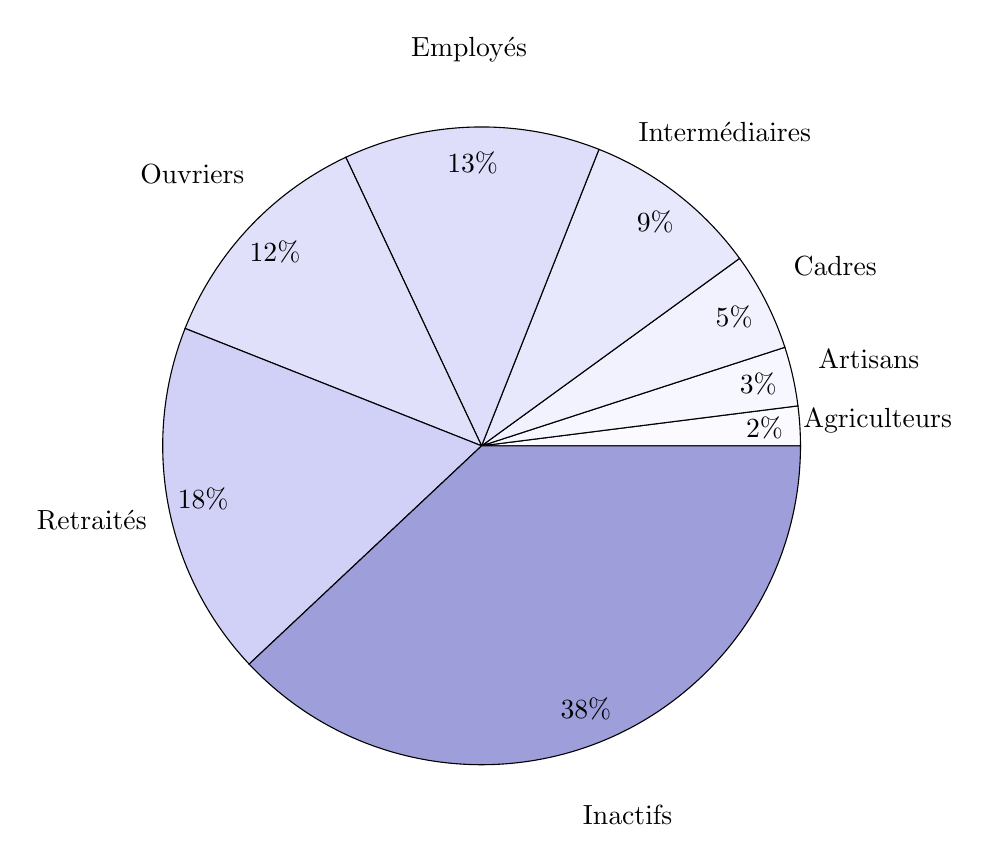
\begin{tikzpicture}[scale=0.9]
\foreach \a/\b/\p/\c in
    {
     0/7.2/2/Agriculteurs, 7.2/18/3/Artisans,
     18/36/5/Cadres, 36/68.4/9/Interm\'ediaires,
     68.4/115.2/13/Employ\'es, 115.2/158.4/12/Ouvriers,
     158.4/223.2/18/Retrait\'es, 223.2/360/38/Inactifs
    }
    {
     \draw[fill=black!\p!blue!\p] (0,0)--(\a: 4.5)arc(\a:\b: 4.5)--cycle; 
     \draw  ({(\a+\b)/2}:4) node {\p\%};
     \draw  ({(\a+\b)/2}:5.6) node {\c};
    } 
\end{tikzpicture}

R\'epartition par cat\'egories socioprofessionnelles en France en 1999
\end{center}

\end{document}
